\appendix
\Chapter{Relációs adatmodell ábrák}

\begin{figure}[H]
    \centering
    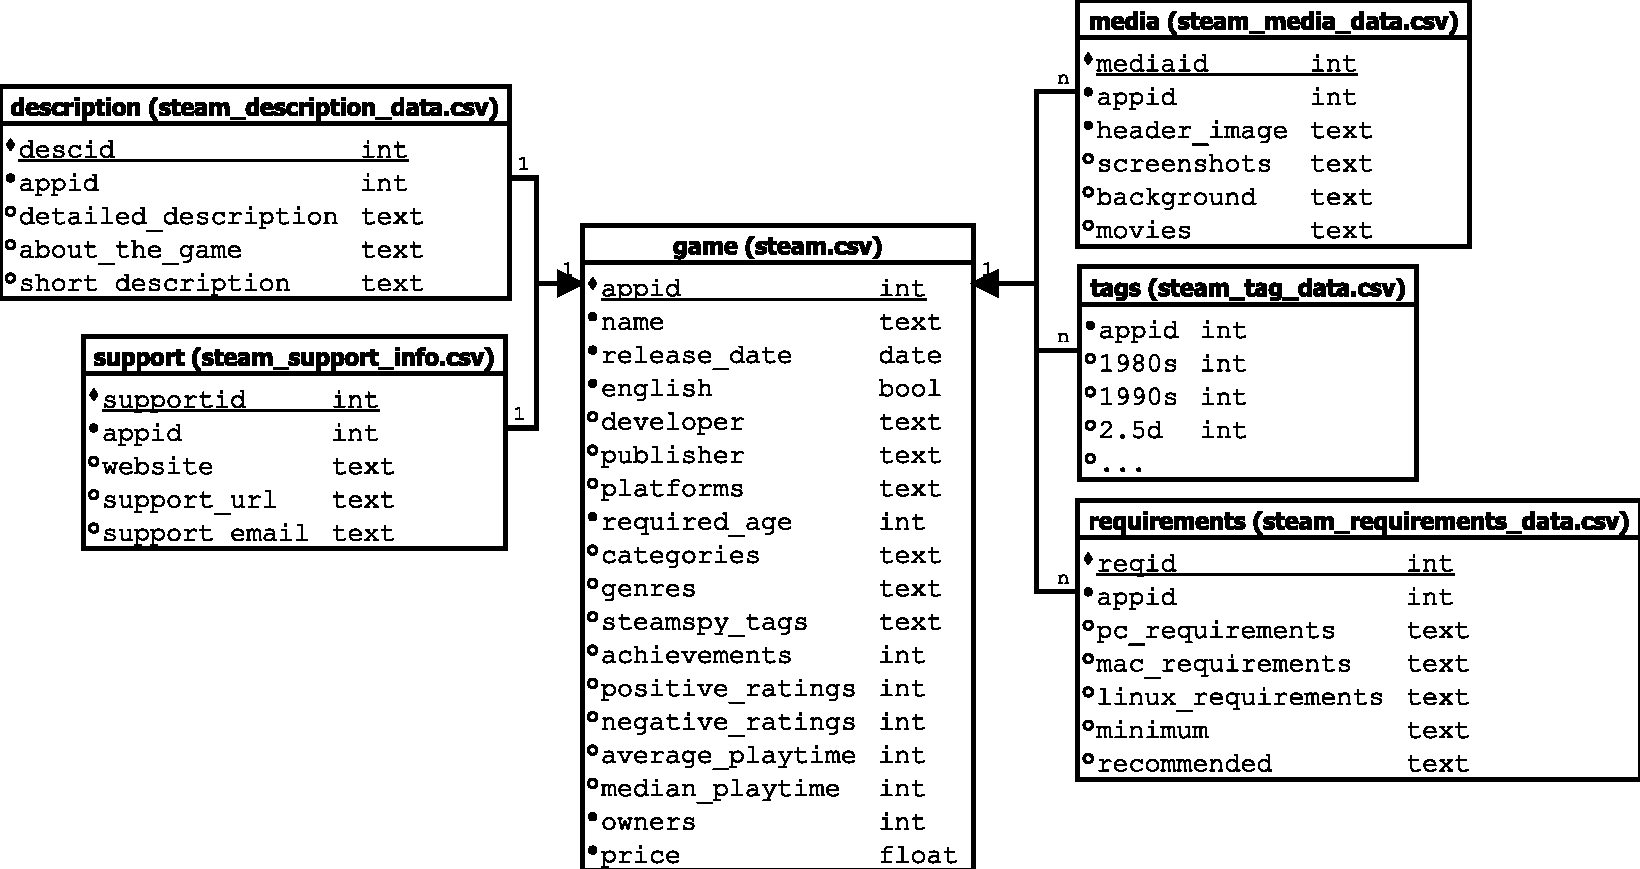
\includegraphics[width=1.0\textwidth]{images/A_unnormalized.pdf}
    \caption{Az A adathalmaz normalizálatlan relációs sémája}
    \label{fig:A_unnormalized}
\end{figure}

\begin{figure}[H]
    \centering
    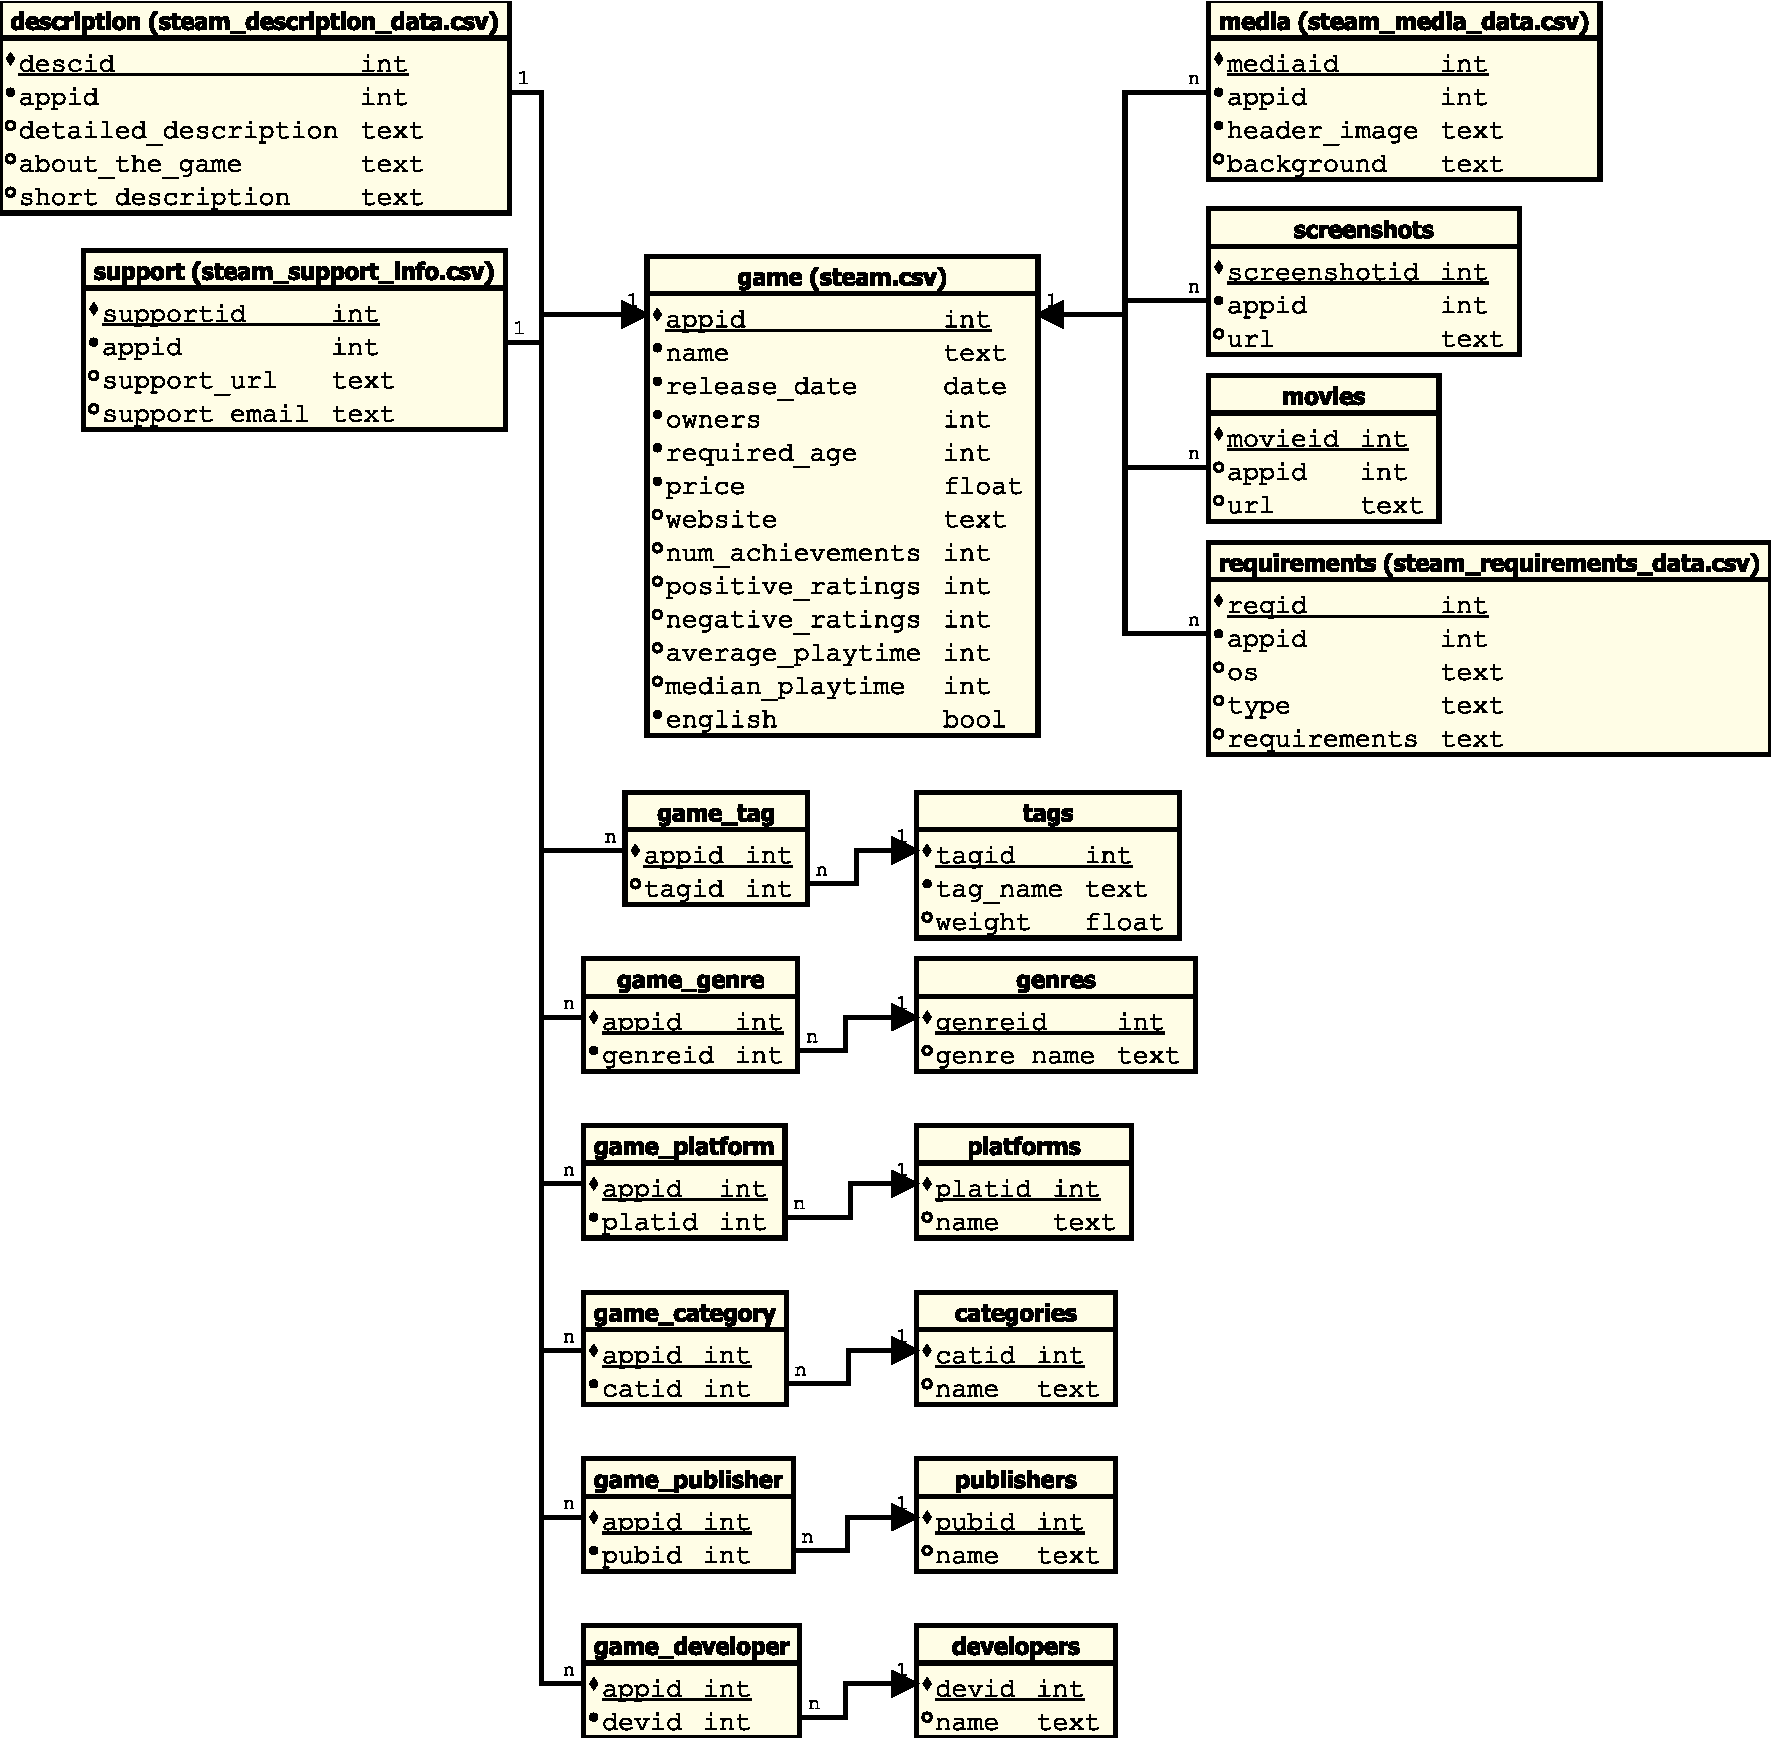
\includegraphics[width=1.0\textwidth]{images/A_normalized.pdf}
    \caption{Az A adathalmaz normalizált relációs sémája}
    \label{fig:A_normalized}
\end{figure}

\begin{figure}[H]
    \centering
    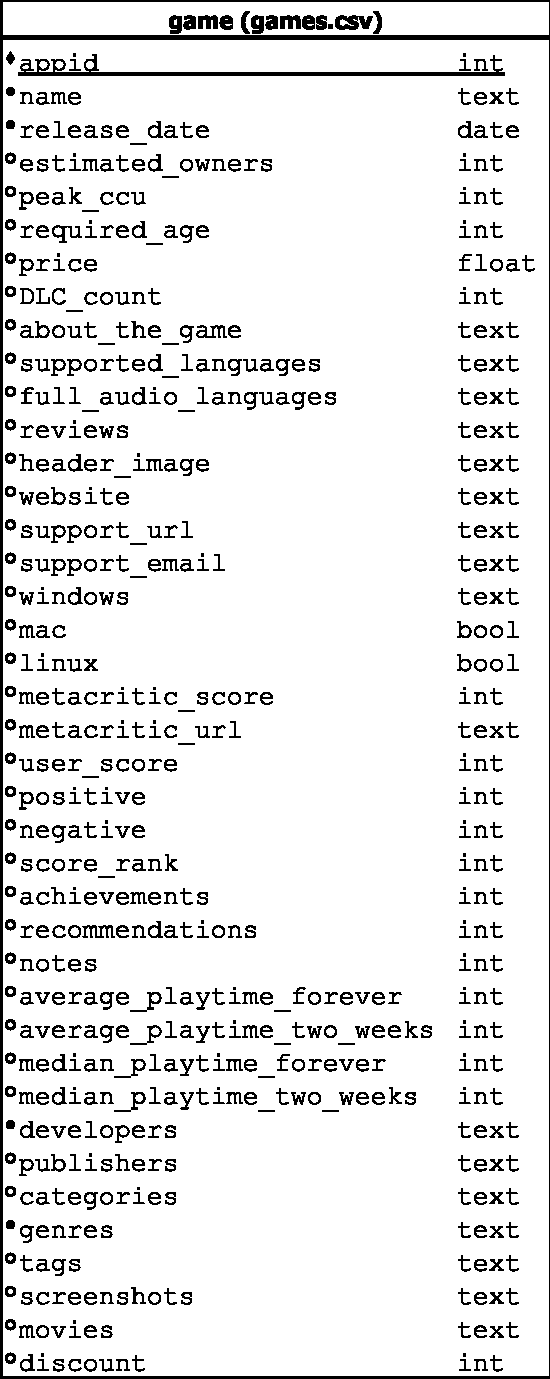
\includegraphics[width=0.6\textwidth]{images/B_unnormalized.pdf}
    \caption{A B adathalmaz normalizálatlan relációs sémája}
    \label{fig:B_unnormalized}
\end{figure}

\begin{figure}[H]
    \centering
    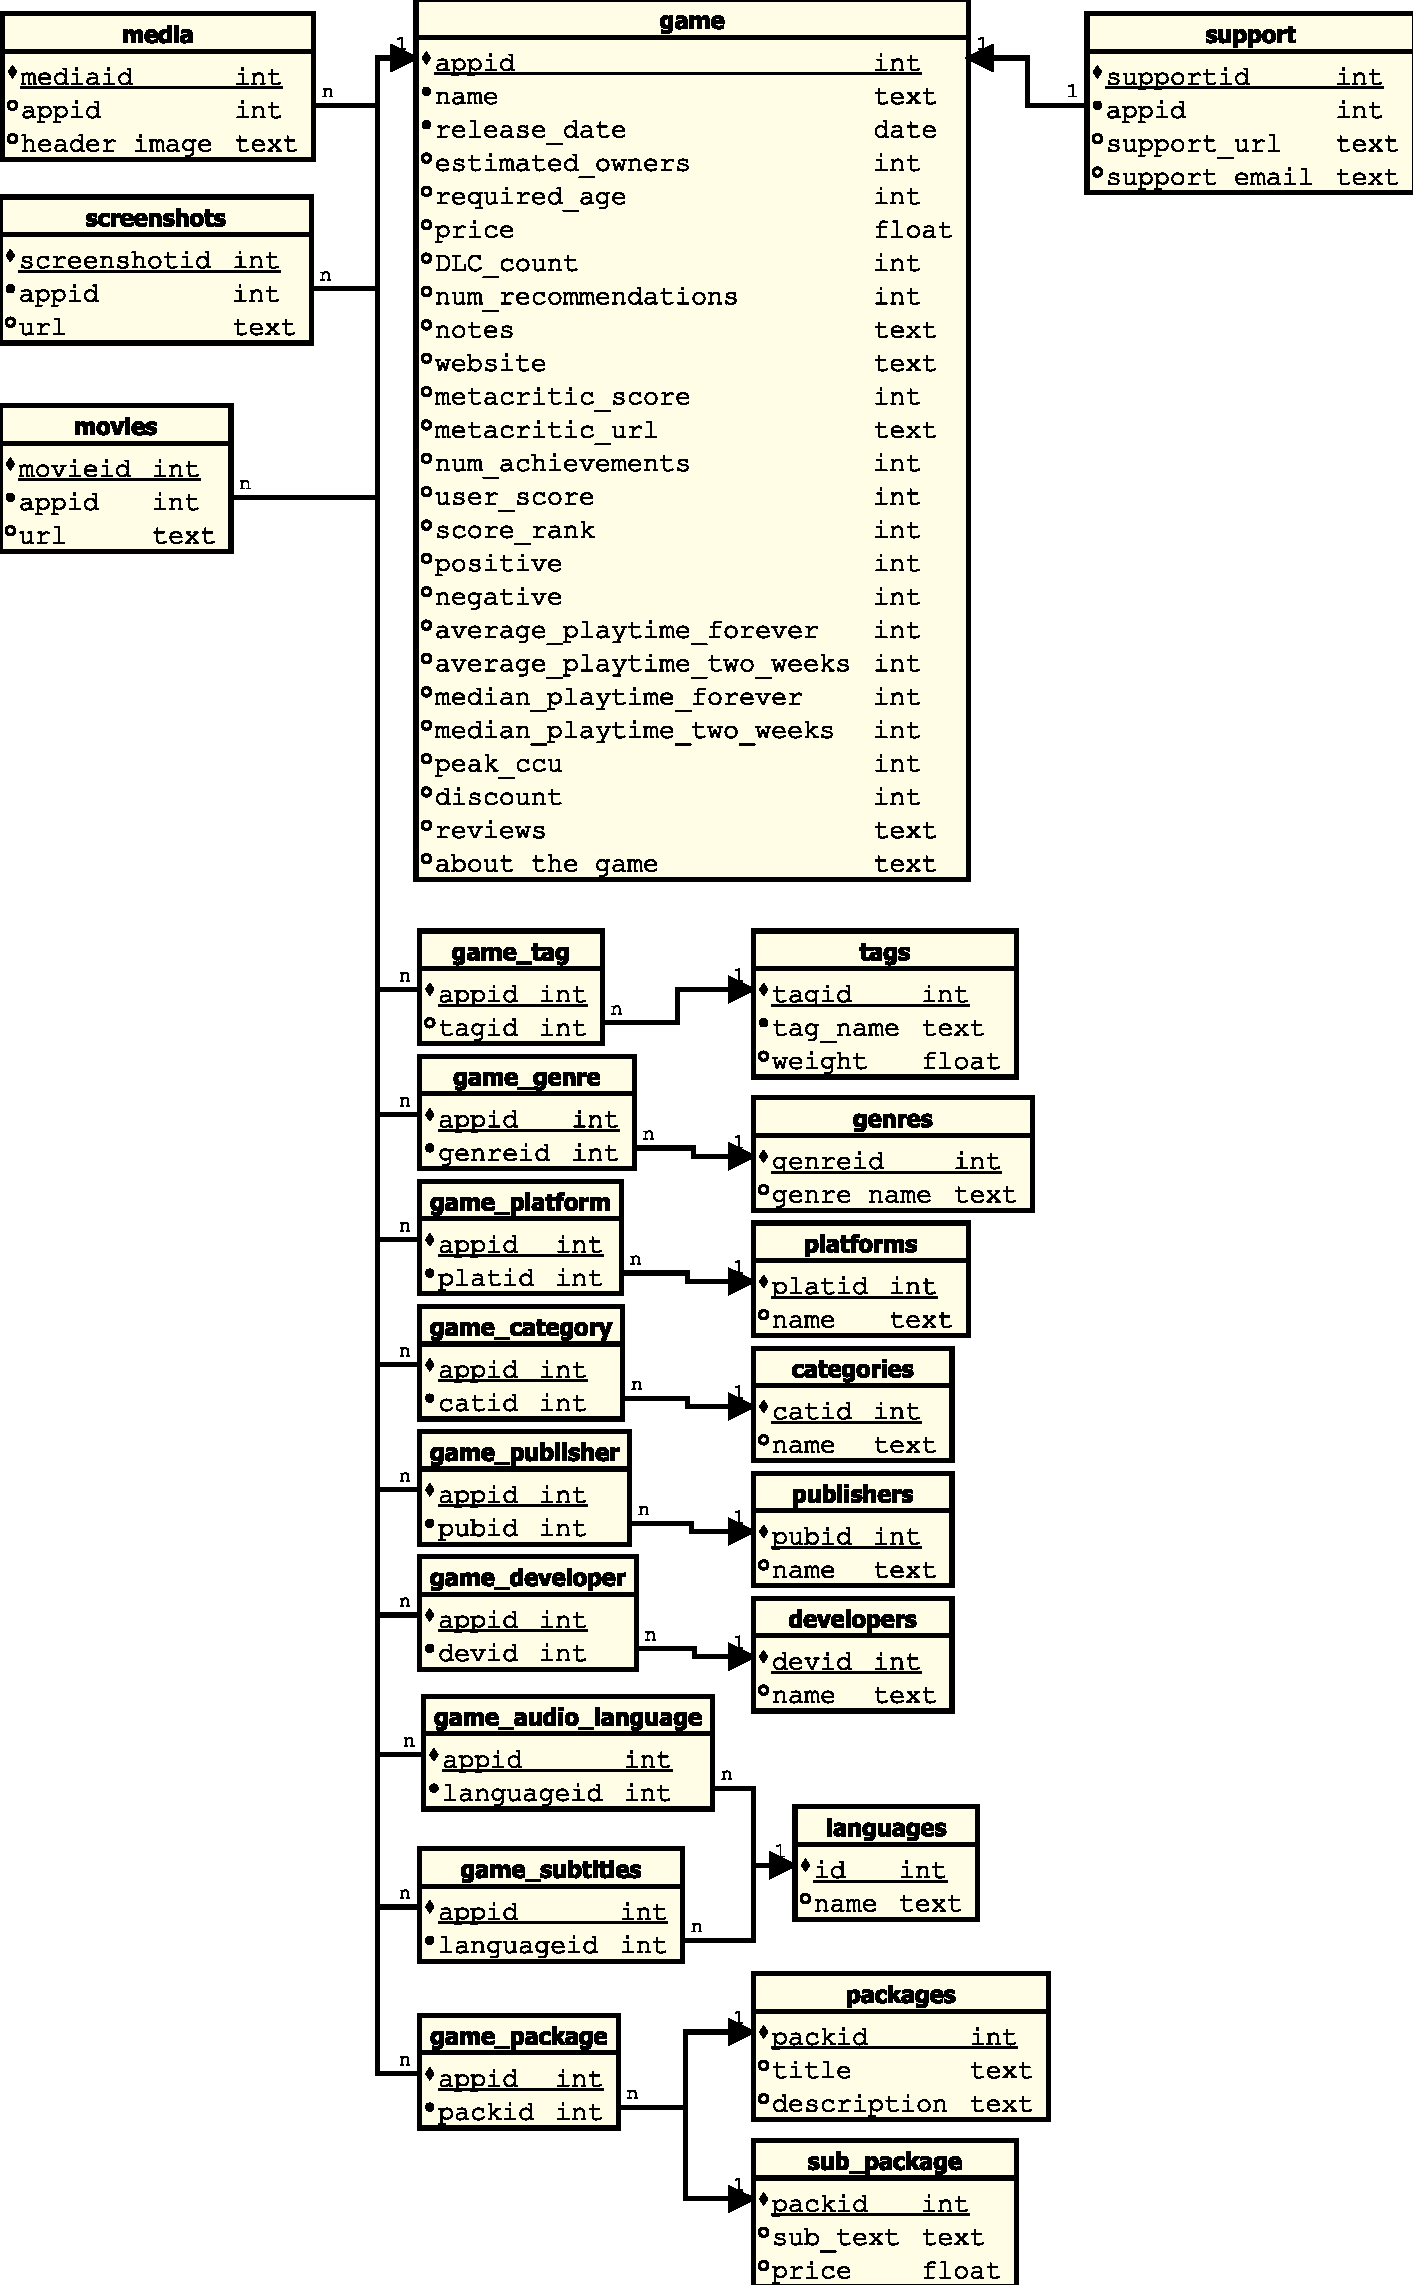
\includegraphics[width=1.0\textwidth]{images/B_normalized.pdf}
    \caption{A B adathalmaz normalizált relációs sémája}
    \label{fig:B_normalized}
\end{figure}

\begin{figure}[H]
    \centering
    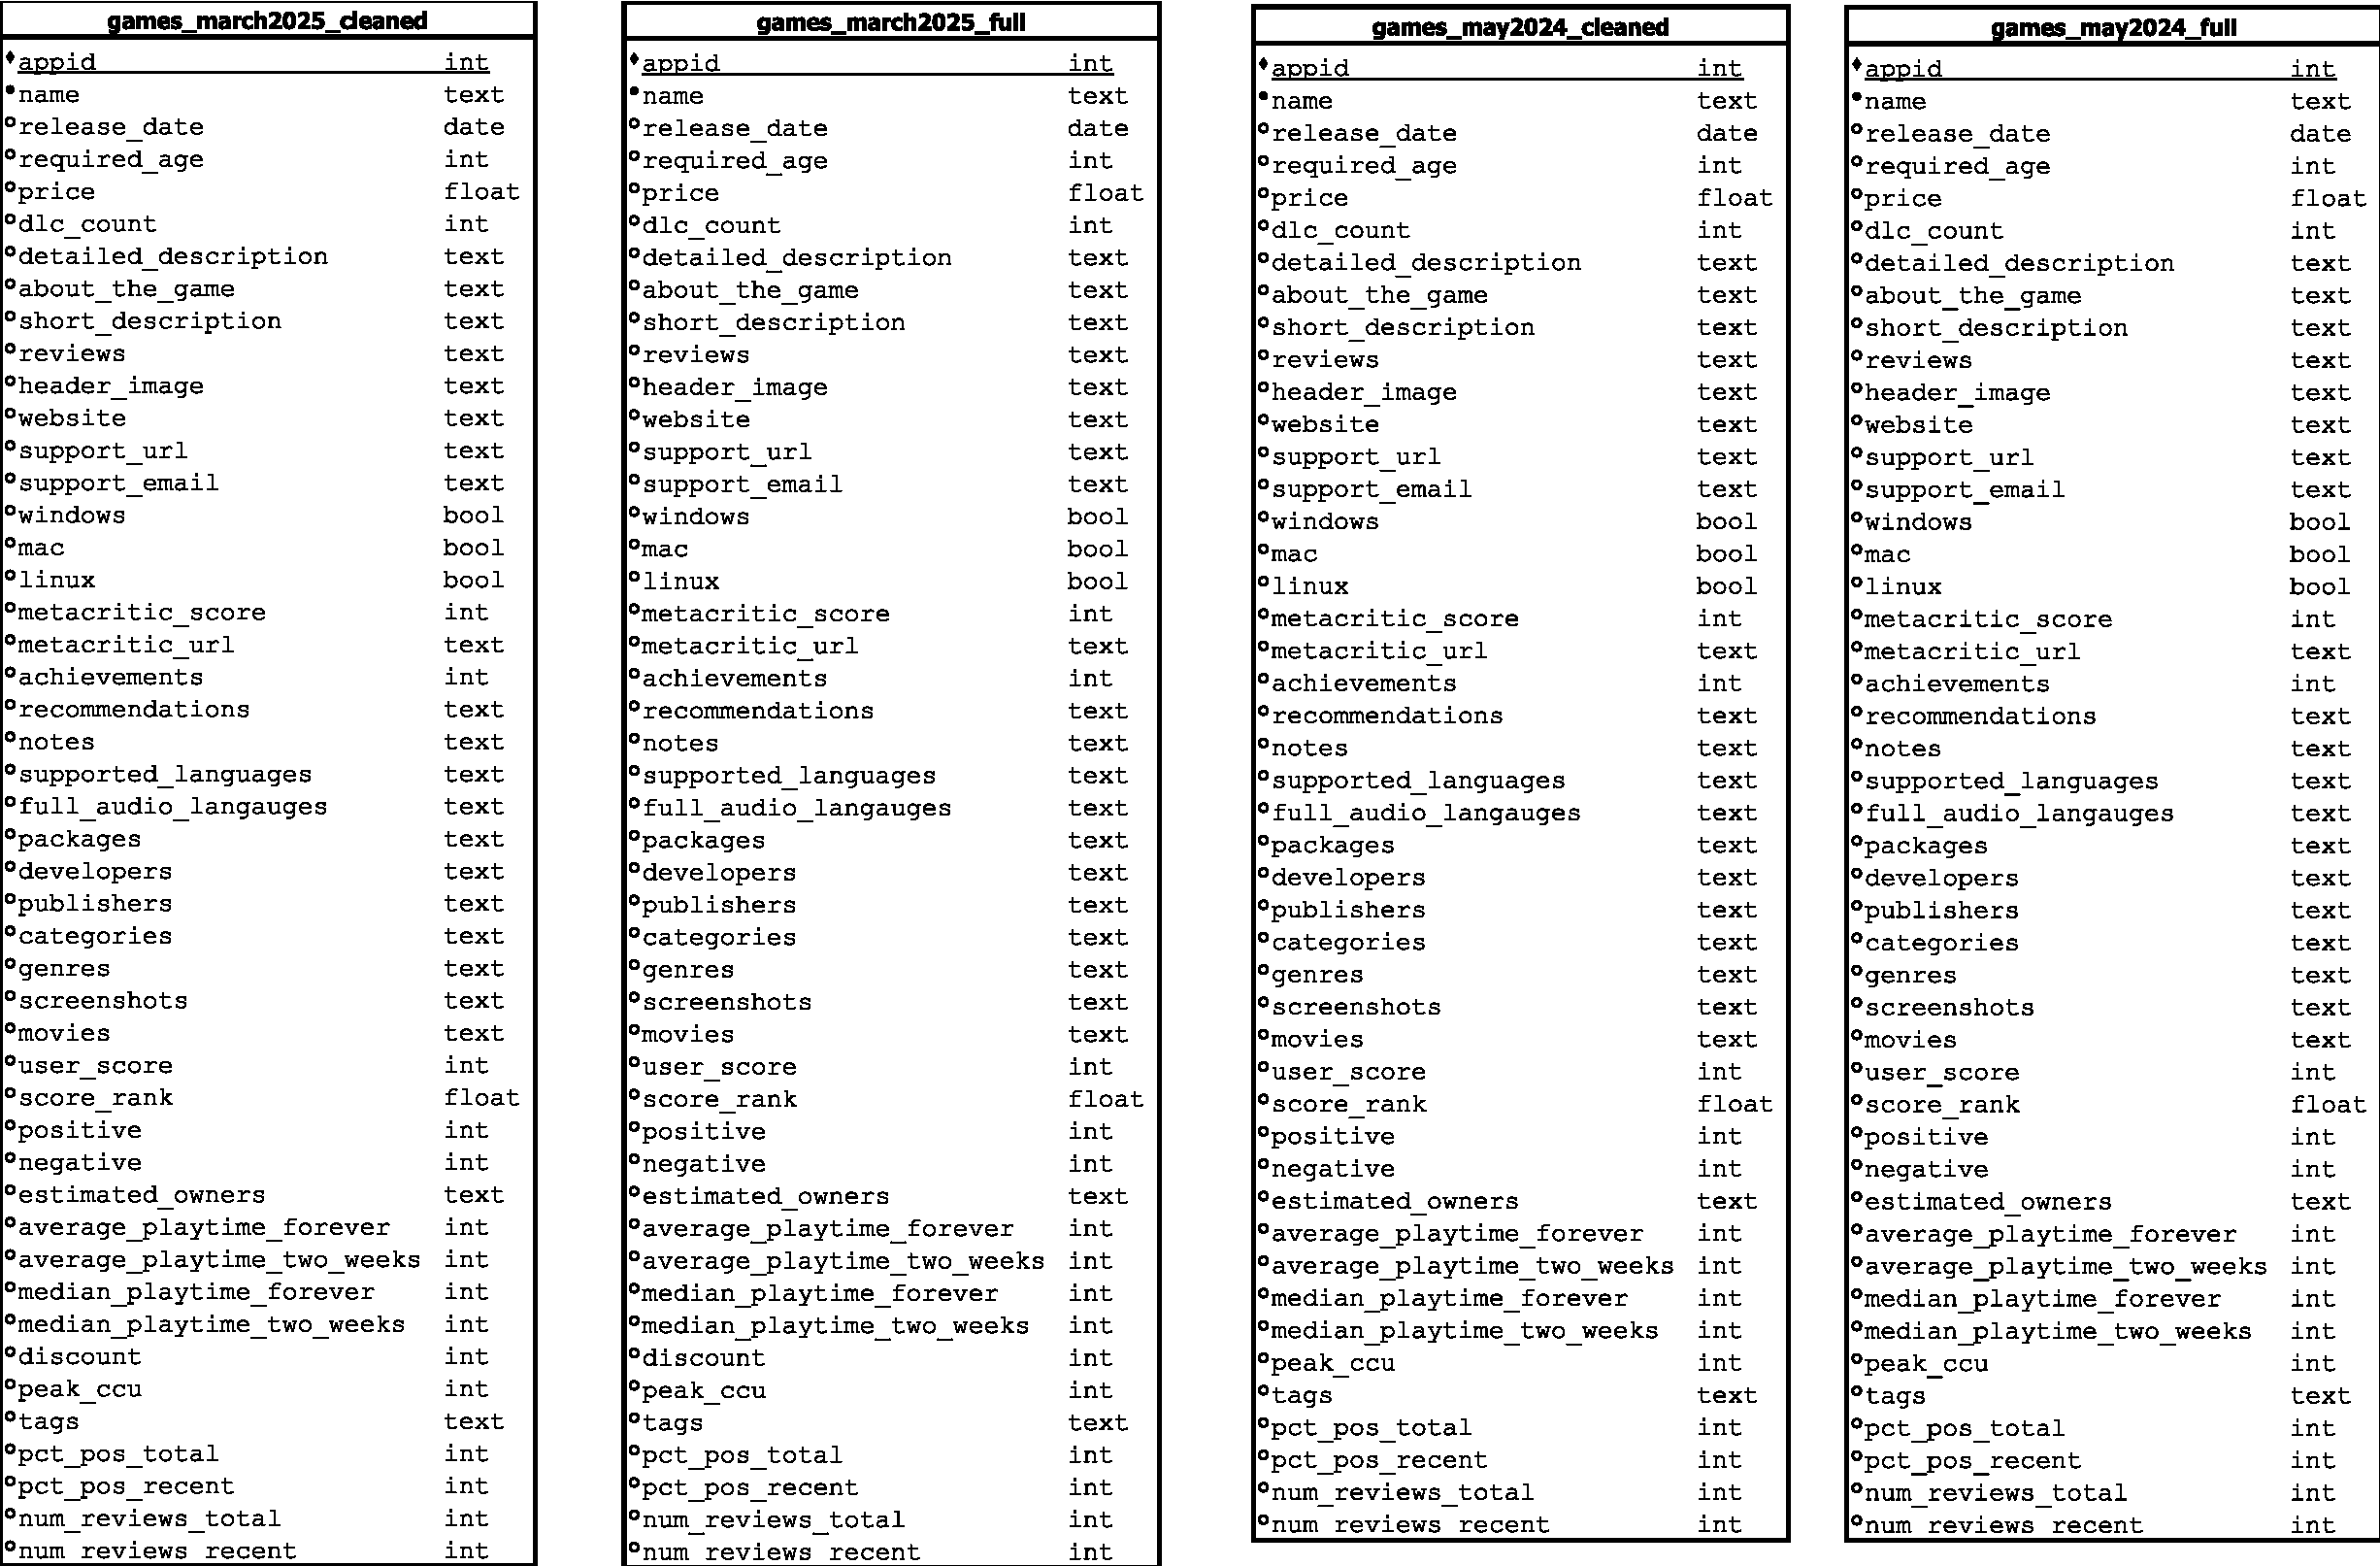
\includegraphics[width=1.0\textwidth]{images/C_unnormalized.pdf}
    \caption{A C adathalmaz normalizálatlan relációs sémája}
    \label{fig:C_unnormalized}
\end{figure}

\begin{figure}[H]
    \centering
    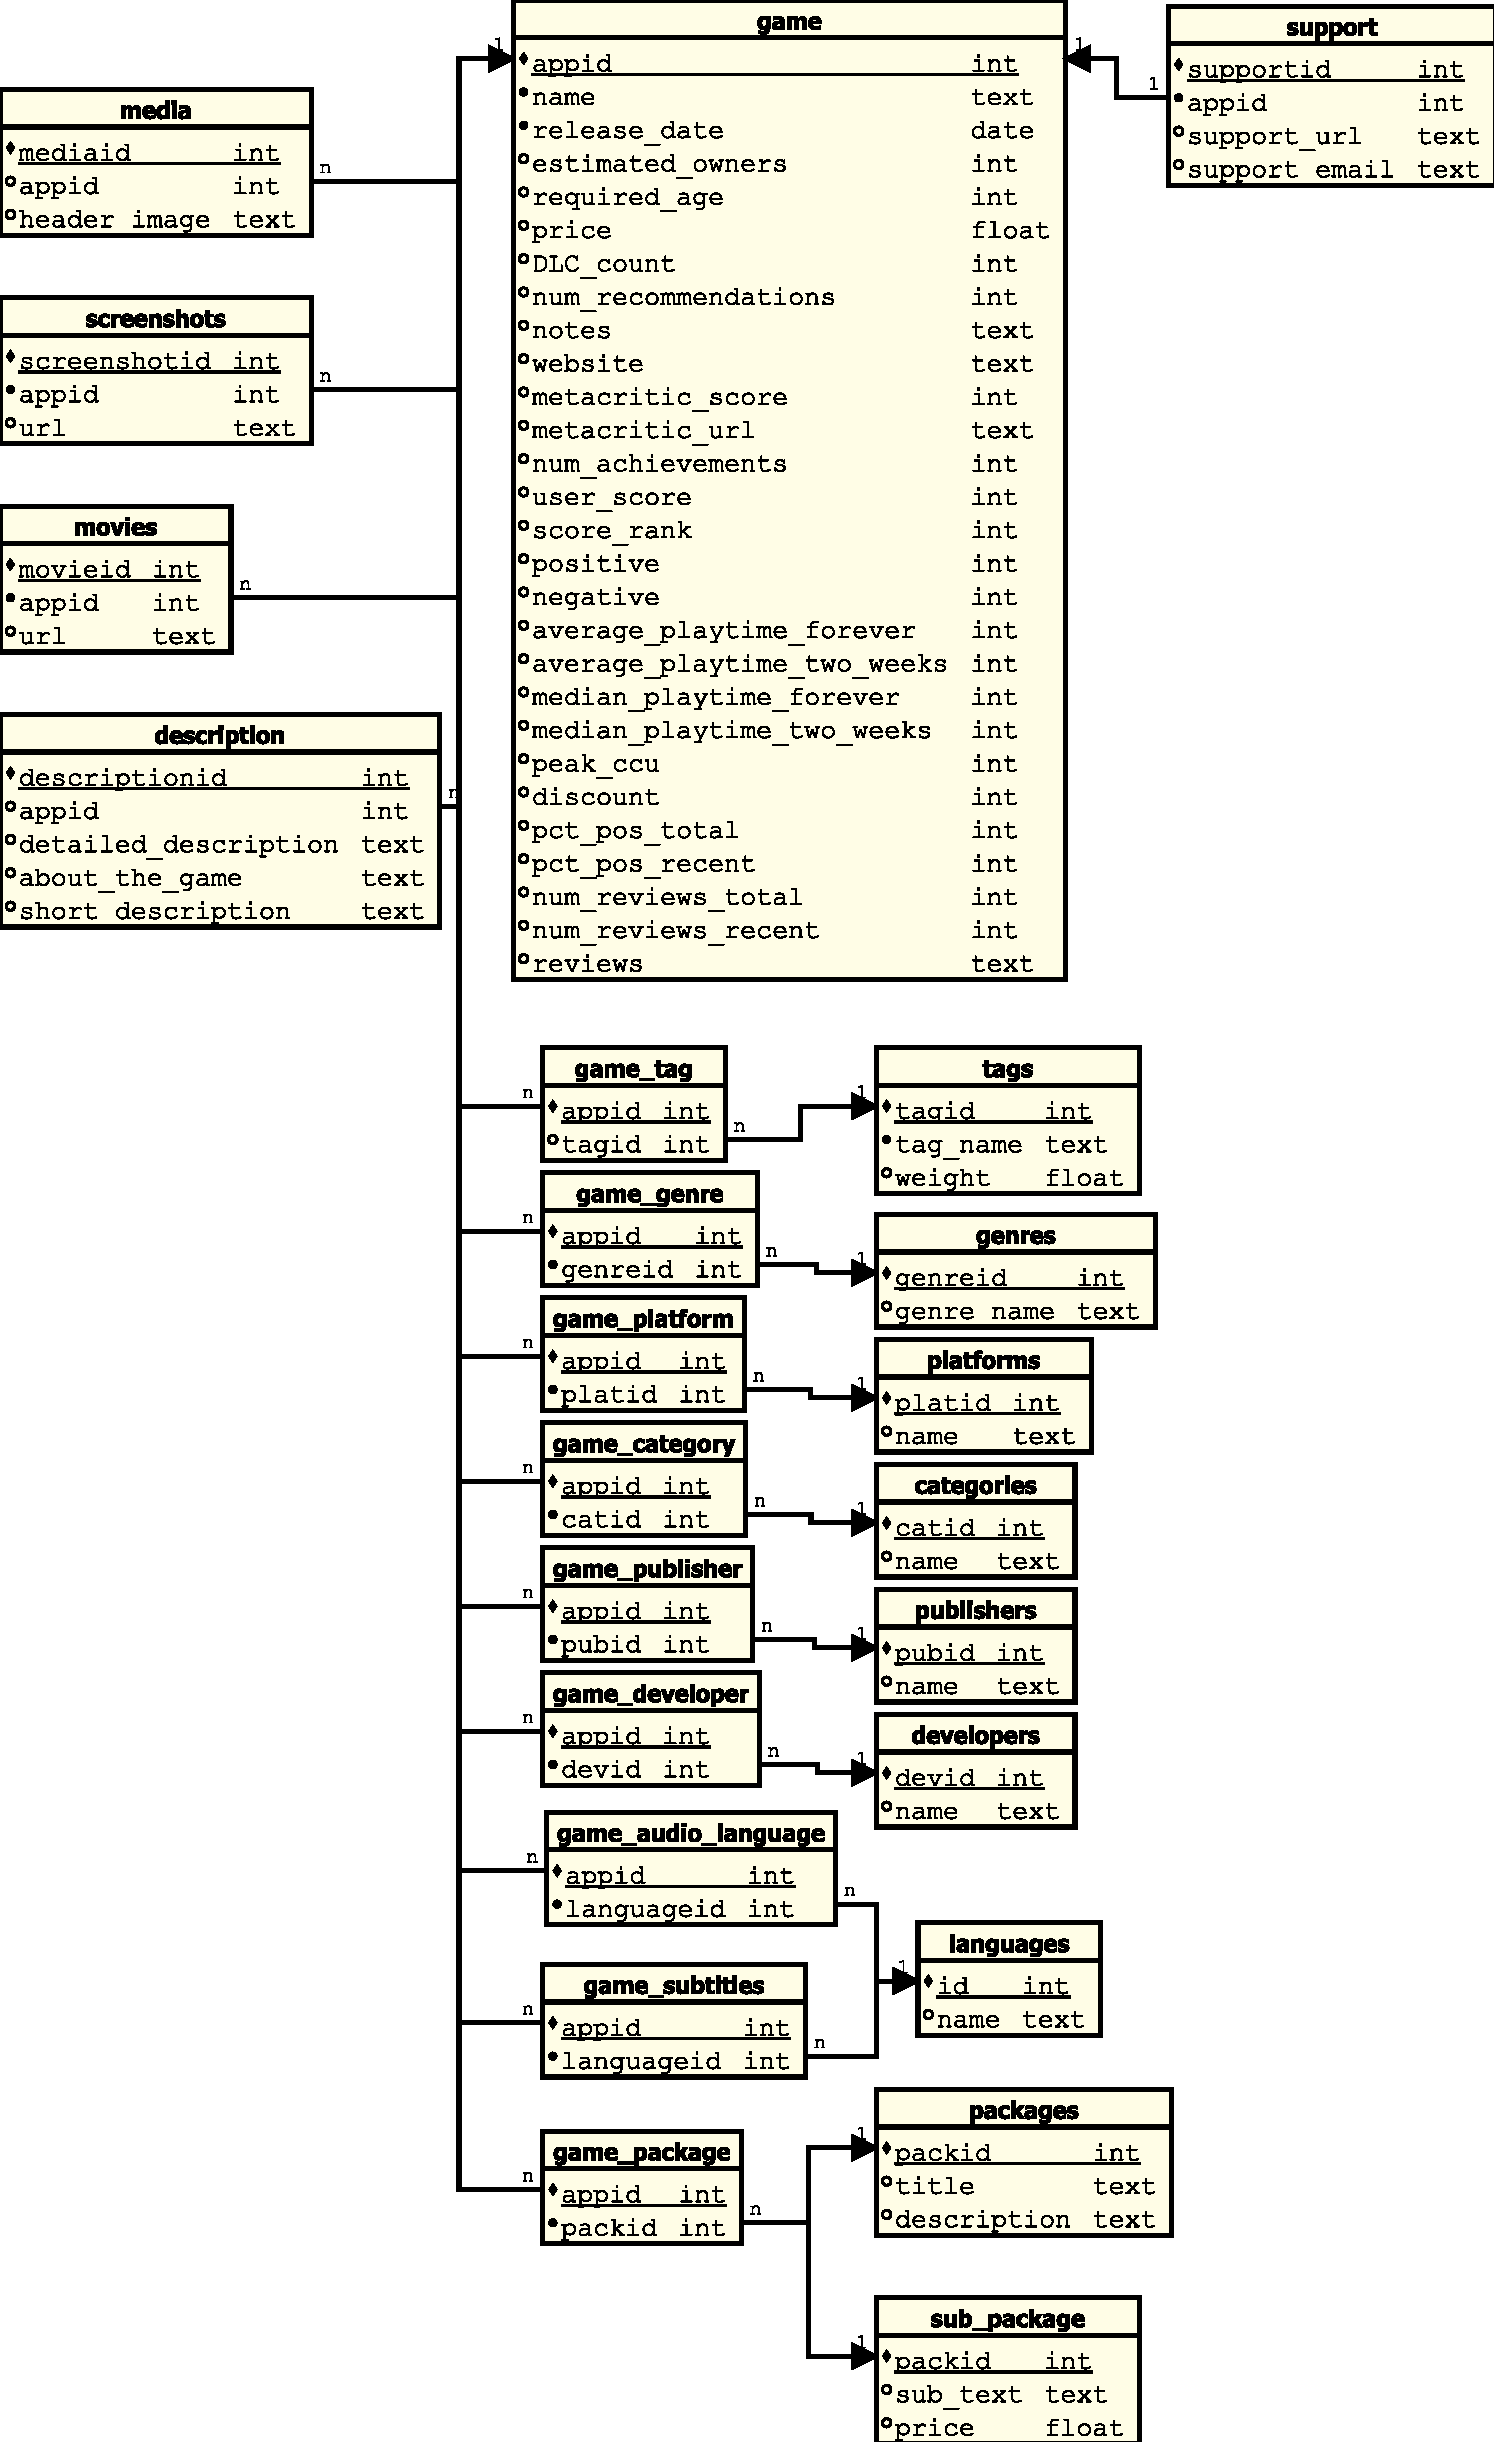
\includegraphics[width=1.0\textwidth]{images/C_normalized.pdf}
    \caption{A C adathalmaz normalizált relációs sémája}
    \label{fig:C_normalized}
\end{figure}

\Chapter{Osztálydiagramok}

\begin{figure}[H]
    \centering
    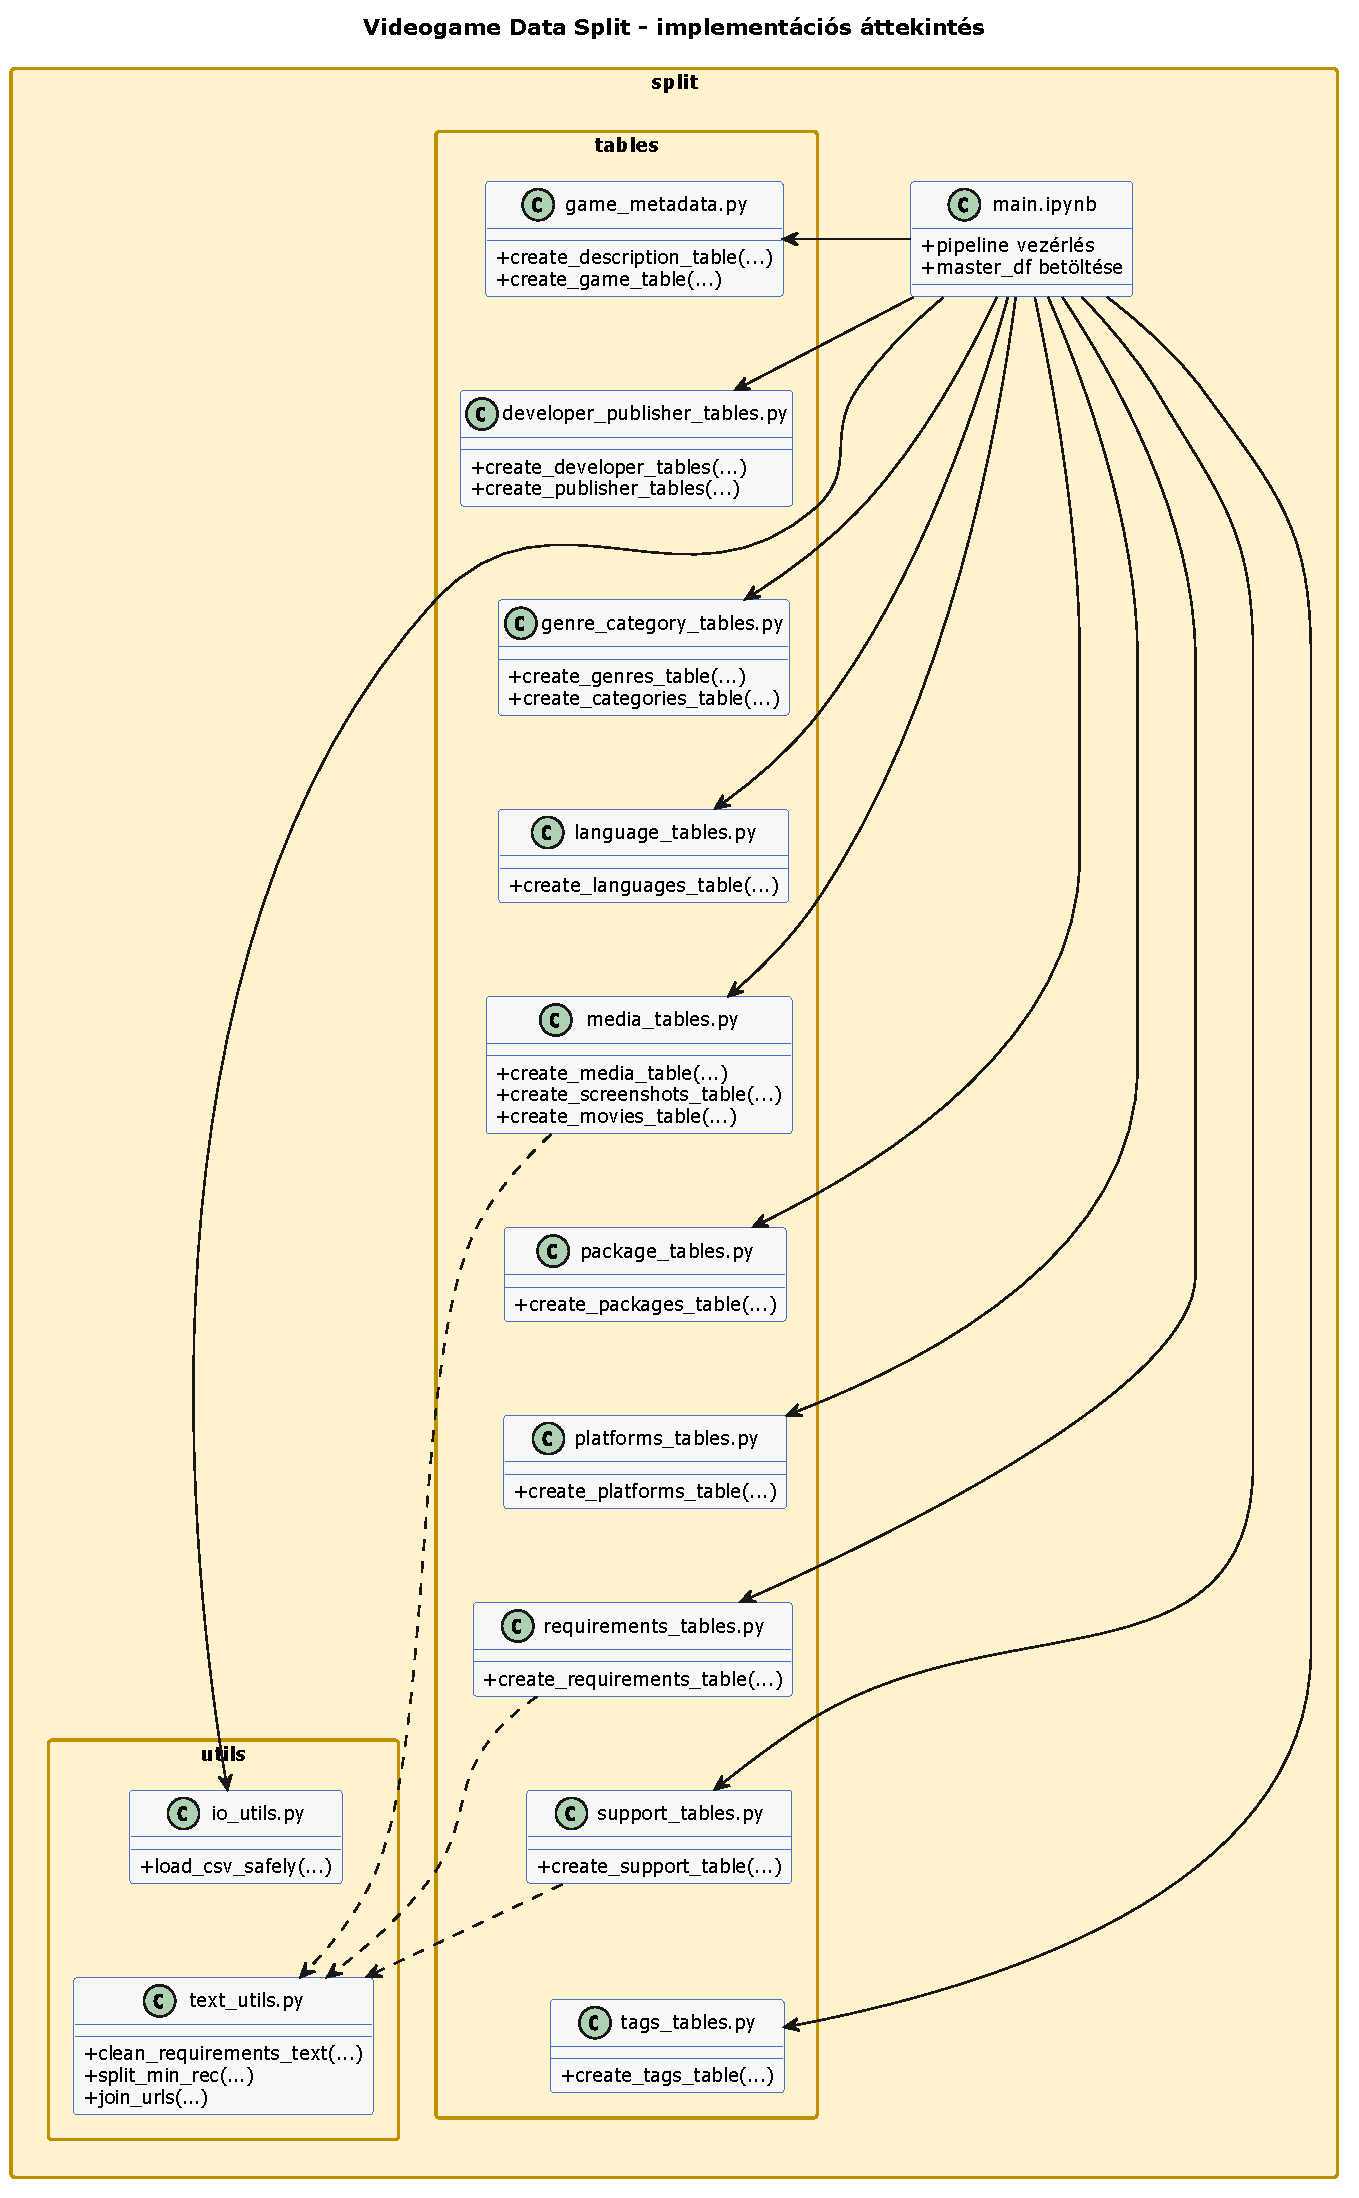
\includegraphics[width=0.9\textwidth]{images/split.pdf}
    \caption{A split implementációs áttekintése}
    \label{fig:split}
\end{figure}

\begin{figure}[H]
    \centering
    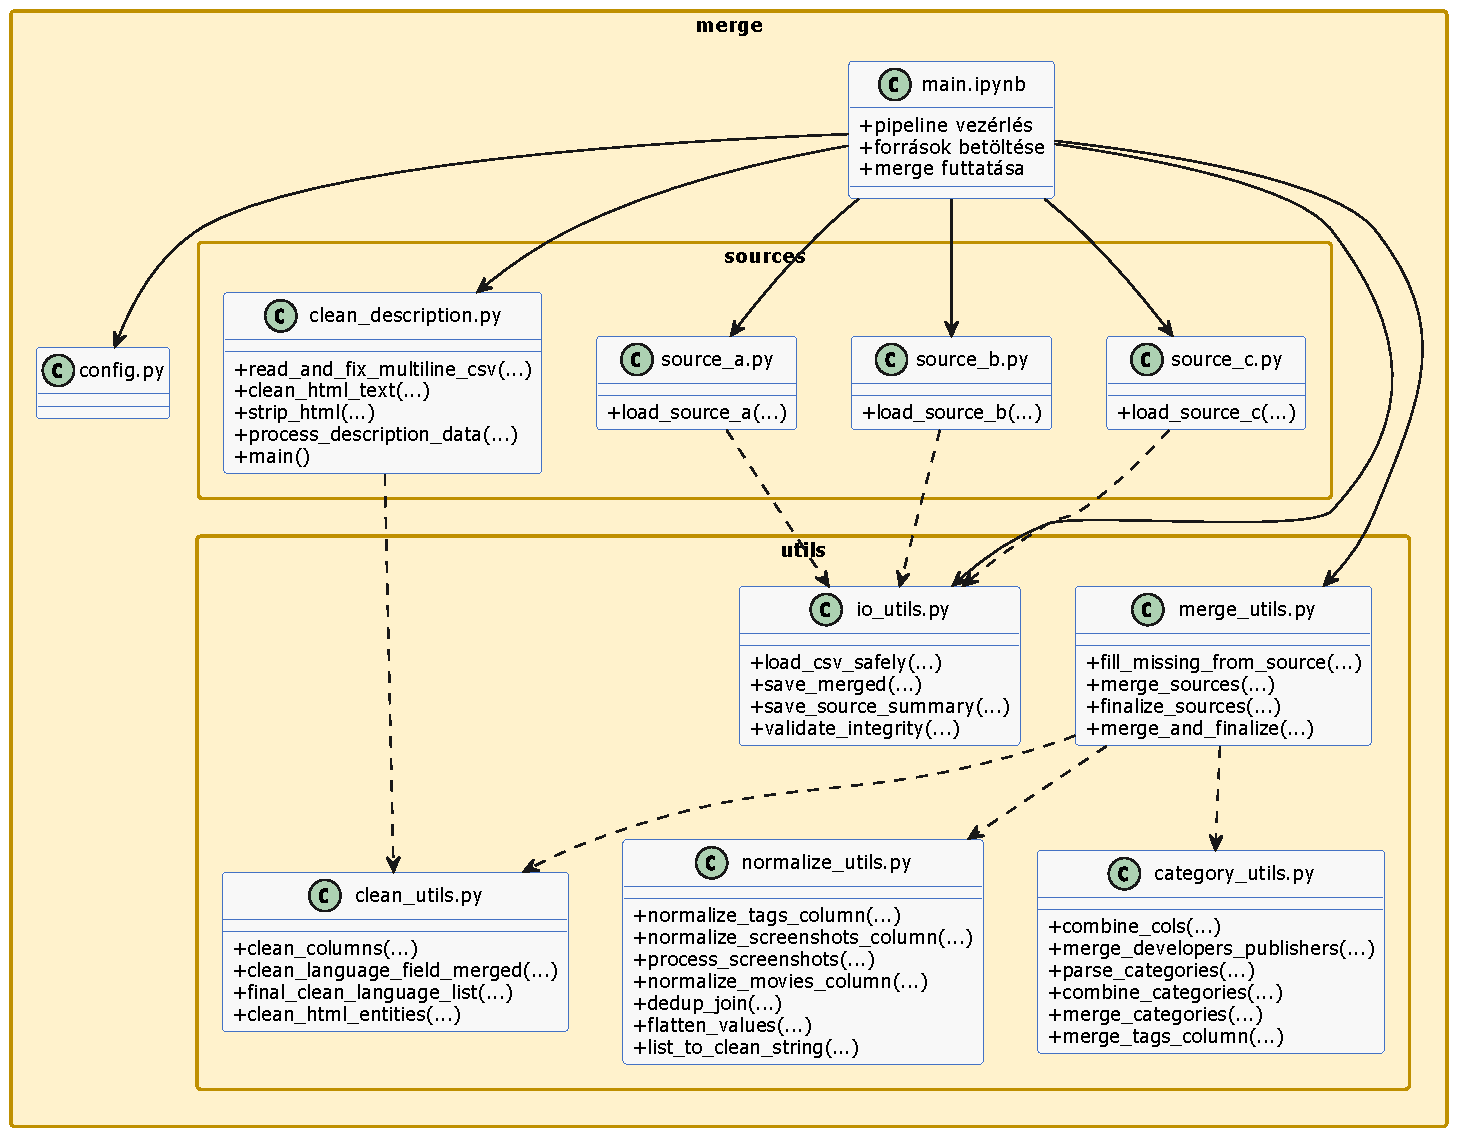
\includegraphics[width=1.0\textwidth]{images/merge_implementation.pdf}
    \caption{A merge implementációs áttekintése}
    \label{fig:merge}
\end{figure}

\begin{figure}[H]
    \centering
    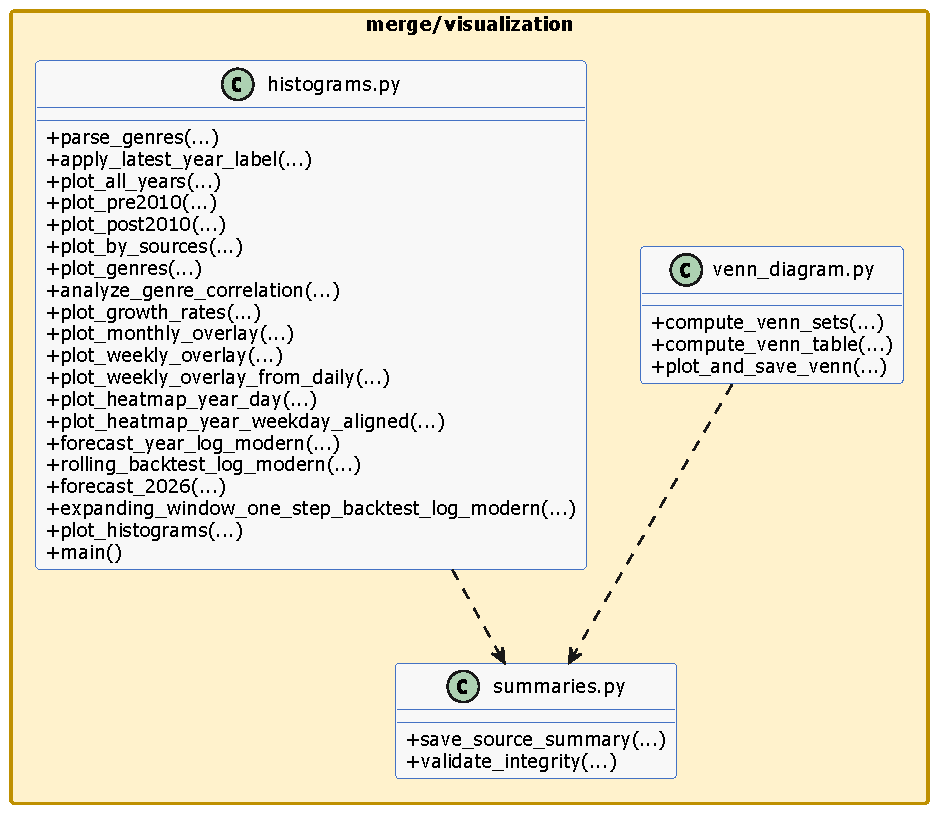
\includegraphics[width=1.0\textwidth]{images/merge_visualization.pdf}
    \caption{A merge vizualizációs áttekintése}
    \label{fig:merge_visualization}
\end{figure}